\documentclass[11pt]{article}

\usepackage{geometry, amsmath, amsthm, latexsym, amssymb, graphicx, hyperref, setspace, color, wasysym}
\usepackage{enumerate}
\geometry{margin=1in, headsep=0.25in}

\parindent 0in
\parskip 12pt

\title{Personalized Highlights Recommendation System}
\author{Muhammad Talha Khan \{Roll \#18100267 \}\\Ahmed Muqaddas \{Roll \#16030039 \}\\Syed Mohsin Bukhari \{Roll \#16030038 \}}
\begin{document}
\maketitle

\section{General Information about data}
\paragraph{}
When there is a cricket or football match going on, there are tweets related to certain hashtags. This data is generated on user's Twitter profile. This kind of data can be streamed live when the matches are going on. Twitter's Streaming API is for this purpose.
\paragraph{}
To the best of our knowledge there is no work done regarding recommending personalized highlights for an event or stream. However, there has been work to detect highlights.\\
\textit{Lanagan, James and Smeaton, Alan F. Using Twitter to Detect and Tag Important Events in Live Sports. Proceedings of the Fifth International AAAI Conference on Weblogs and Social Media, 2011}
\paragraph{}
Collected tweets are mostly text. Further processing is required to extract insights from this text data. Sentiment for each tweet has to be extracted and then the data has to be restructured in form of a matrix. This will help fill out missing values and predict sentiment of new streams for users.
\paragraph{}
A single data object corresponds to a tweet which is a sentiment score of a user at a particular time. This object will be processed and it will correspond to an element in a matrix where rows are users and columns are time slot of highlights.
\paragraph{}
The data is in form of streams. Data is captured on the go. That's nature of the problem. However, the dataset needed for sentiment analysis is available and downloaded. The size of one data stream is typically 2MB to 10MB. The overall size of the data is not known and irrelevant because the analysis that is performed needs a stream of data and does not require to data other than what the algorithm produces itself.
\paragraph{}
Each stream of data is four dimensional. One dimension corresponds to users, the other to different streams, the third to time and the fourth to sentiment embedded in the tweet. However, for preprocessing each data object in order to perform sentiment analysis, the dimension of data is the number of words in vocabulary. This is typically between ten to thirty thousand. For now, we will stick to the lower bound of the range, i.e. ten thousand. Other size related properties include the length of each tweet, which Twitter allows to be 240 characters. This means that a typical Tweet has between 25 to 50 words.

\section{Data Format, Types and Description}
\begin{itemize}
	\item The file type is \textit{.txt} for both streamed data and unstructured text data.
	\item For streams the algorithm stores following attributes.
	\begin{itemize}
		\item user\_id (to identify user)
		\item tweet\_id (to identify tweet and fetch more data if needed in future)
		\item tweet\_content (the content of the tweet to perform analysis on)
		\item date\_time (time at which tweet was Tweet was generated)
	\end{itemize}
	\item Detailed description of data\\
	There are typically ten to twenty thousand tweets for a PSL cricket match. The data for Personalized Highlights Recommendation System needs to be four dimensional. However, each data object from the stream needs to be preprocessed in order to represent it in the desired four dimensions (users, streams, time, sentiment).
	
	\begin{itemize}
		\item Data types and description of each feature:\\
		\begin{tabular}[ht]{|l|l|l|}
			\hline
			\textbf{Attribute} & \textbf{Data Type} & \textbf{Description}\\
			\hline
			user\_id & Numerical & Unique identifier for a user\\
			tweet\_id & Numerical & Unique identifier for a tweet\\
			tweet\_content & Text & The actual content that is used to determine embedded sentiment\\
			date\_time & DateTime & The time at which the tweet was generated\\
			\hline
		\end{tabular}
		\item Data types and description of each dimension:\\
		\begin{tabular}[ht]{|l|l|l|}
			\hline
			\textbf{Dimension} & \textbf{Data Type} & \textbf{Description}\\
			\hline
			user\_id & Numerical & Unique identifier for a user\\
			stream\_id & Numerical & Unique identifier for a stream\\
			sentiment & Numerical & A number representing sentiment of a user at this particular time\\
			date\_time & Numerical & The time at which the sentiment was generated\\
			\hline
		\end{tabular}
	\end{itemize}
	\item Each data object is a tweet, therefore, for sentiment analysis, tweet specific grammar and vocabulary must be used. This grammar and vocabulary is very different from that of actual language.
\end{itemize}

\section{Data preprocessing}
\paragraph{}
The tweets have to be processed in order to extract sentiment from them. Each tweet has to go through a pipeline to be available for sentiment extraction.
\begin{enumerate}[1.]
	\item Stopword Removal
	\item Lemmatization
	\item Drop very common and rare words
\end{enumerate}
After these steps, each tweet can be expressed as a vector of TF-IDF values where each element corresponds to one word. An alternative to this can be the usage of word embeddings like \textit{Word2Vec} or \textit{GLoVe}.
\paragraph{}
There will be a lot of missing data once the sentiment has been extracted. For this, a search will be required for similar users and similar streams in order to fill in the missing values.
\paragraph{}
There might be some noise in the data. In order to deal with that, there can be a range of techniques that can be used to detect this noise. For example, histogram of words can be matched or Hamming distance can be computed to find outliers.

\section{EDA}
There are no numerical attributes in this dataset for which measures of centrality and spread need to calculated at this stage of the analysis. However, histograms for number of tweets can be plotted along time axis. It is clearly visible that there are some humps in the histogram. These events correspond to the real time highlights when something important happened in the match.

\begin{figure}[ht]
	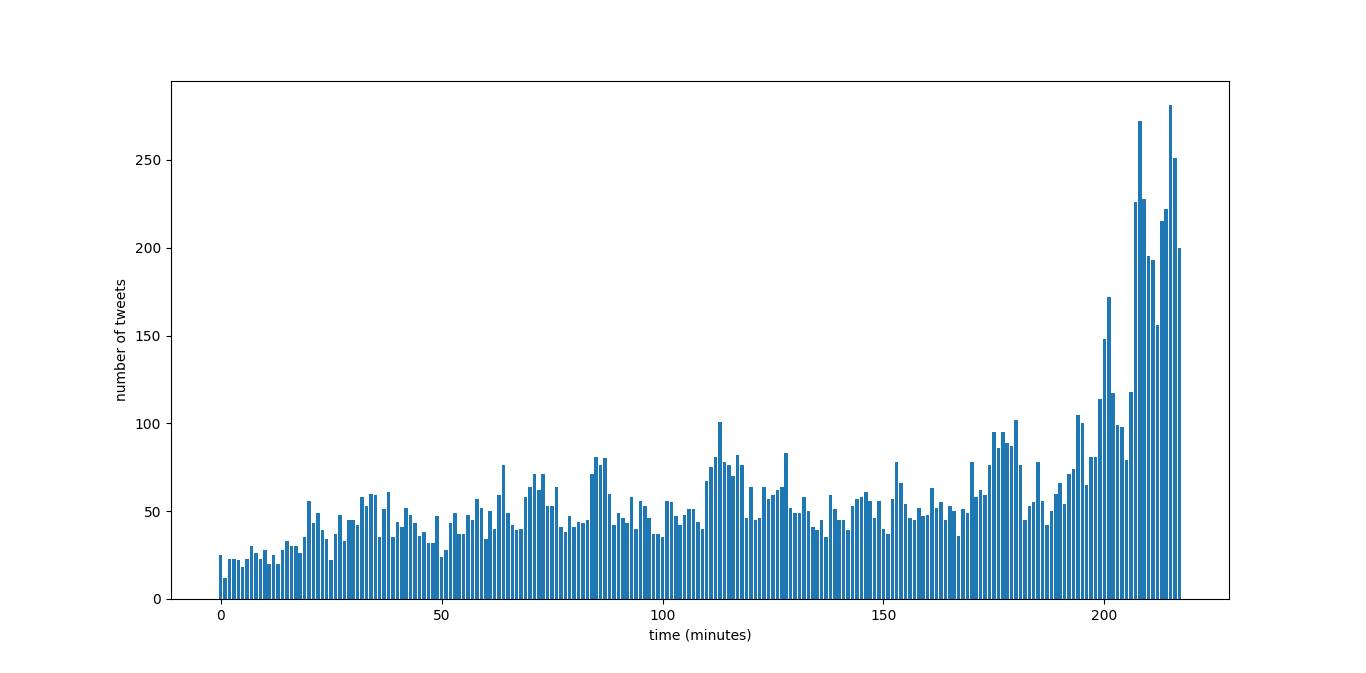
\includegraphics[scale=0.35]{/home/elcid/workspace/stream_analytics/docs/figs/match_01.jpg}
	\caption{Match 1 (16th March, 2018)}
\end{figure}
\begin{figure}[ht]
	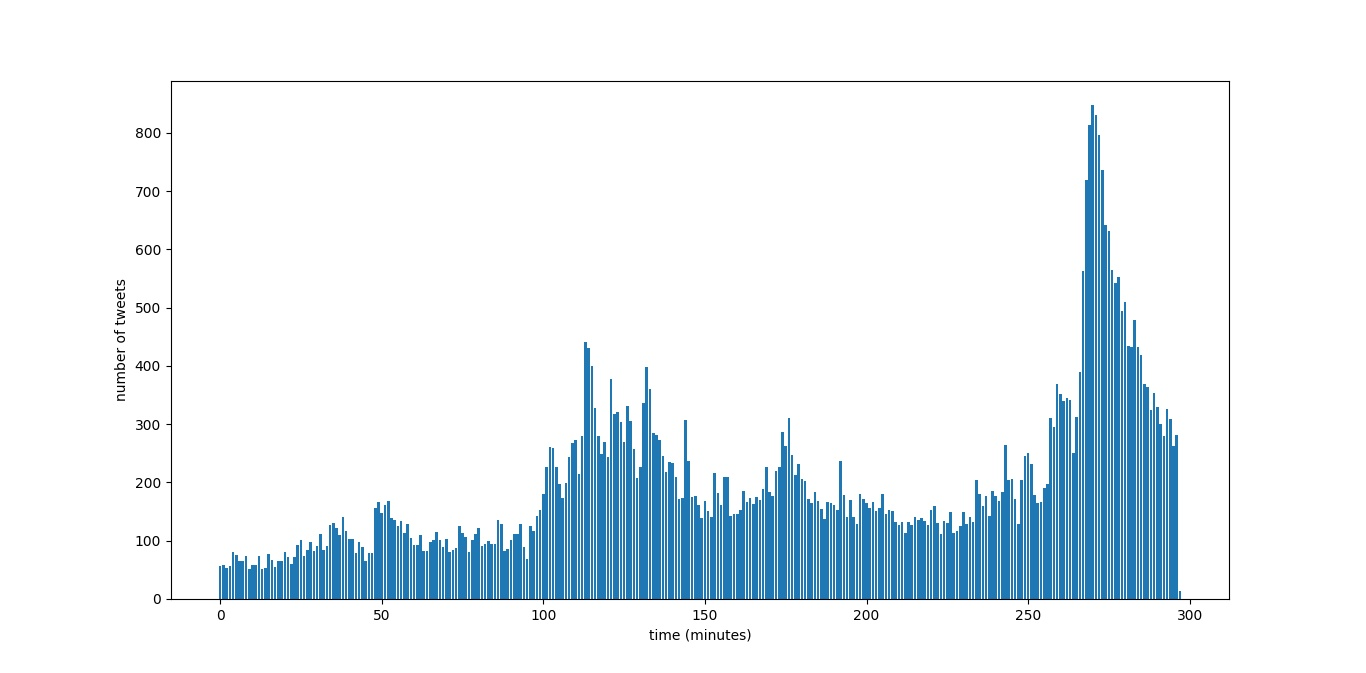
\includegraphics[scale=0.35]{/home/elcid/workspace/stream_analytics/docs/figs/match_02.jpg}
	\caption{Match 2 (21st March, 2018)}
\end{figure}
	
\end{document}
